\chapter{تطبيقات}

\section{معادلة الحركة \en{Equation of Motion}}

من قانون نيوتن الثاني لحركة جسم ما 
\begin{equation}
	\label{eq:newton2law}
	\sum \vec{F} = m a
\end{equation}
حيث 
\begin{itemize}
	\item $\sum \vec{F}$ مجموع القوى المؤثرة على الجسم.
	\item $m$ كتلة الجسم.
	\item $a$ تسارع الجسم ($a = \dfrac{d^2 y}{dt^2}$)
\end{itemize}

\begin{english}
	\begin{figure}[ht]
	\centering
	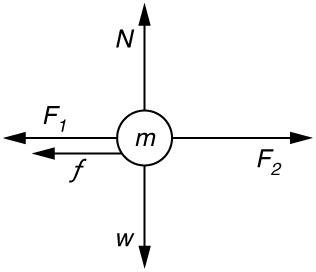
\includegraphics[width=0.3\textwidth]{Figures/em.jpg}
	\caption{Equation of motion}
\end{figure}
\end{english}

نطبق هذه المعادلة على سقوط حر لجسم (نهمل قوة مقاومة الهواء) اذن هناك قوة واحدة تؤثر على الجسم وهي (وزن الجسم). يمكن حساب وزن الجسم من خلال القانون 
\[
\vec{F}_w = - mg
\]
حيث $g$ تعجيل الجاذبية الارضي. اذن بالتعويض في \eqref{eq:newton2law} نحصل على 
\begin{equation}
	\label{eq:freefall}
	- mg = m \frac{d^2 y}{dt^2} \Rightarrow \frac{d^2 y}{dt^2}  = -g
\end{equation}
مع الشروط الابتدائية
\begin{itemize}
	\item $y(0) = y_0$ موضع السقوط.
	\item $y'(0) = v_0$ السرعة الابتدائية.
\end{itemize}
الآن نطبق تحويل لابلاس على المعادلة وتعويض الشروط الابتدائية
\[
\LL\{y''\} = \LL\{-g\}
\]
\[
s^2Y(s) - s y(0) - y'(0) = \frac{-g}{s} 
\]
\[
Y(s) = \frac{1}{s^2} \left[\frac{-g}{s} + sy_0 + v_0\right]
\]
\[
Y(s) = \frac{-g}{s^3} + \frac{v_0}{s^2} + \frac{y_0}{s}
\]
بتطبيق لابلاس العكسي نحصل على
\begin{equation}
	\label{eq:motionsol}
	y(t) = -\frac{1}{2}gt^2 + v_0 t +y_0
\end{equation}
هذه المعادلة تصف موضع الجسم بعد مرور $t$ من السقوط.\\ \\
\noindent
\textbf{مثال عددي}\\
\noindent
سقط جسم من ارتفاع $y_0 = 100\text{m}$ بسرعة ابتدائية $v_0 = 0 $ المطلوب ايجاد الارتفاع بعد $t = 2\sec$
\begin{solution}
	تعجيل الجاذبية $g = 9.8 \text{m}/\sec^2$ اذن
	\[
	y(2) = -\frac{1}{2} \times 9.8 \times (2)^2 + 0 \times 2 + 100 = 80.4 \text{m}
	\]
\end{solution}

\section{معادلة تدفق بوازوي \en{Poiseuille's Flow Equation}}
يعد قانون بوازوي من القوانين الاساسية في ميكانيكا الموائع. حيث يصف تدفق الموائع اللزجة داخل الانابيب الدقيقة. لكي نشتق هذا القانون نستخدم من معادلات نافير ستوكس \\(\en{Navier Stokes Equations}) للحالة الخاصة بتدفق طبقي منتظم لسائل لزج داخل انبوب اسطواني افقي.\\
\noindent
\textbf{الفرضيات}
\begin{itemize}
	\item السريان ثابت (لا يوجد تغير زمني).
	\item السريان طبقي ومتناظر حول محور الانبوب.
	\item السائل غير قابل للانضغاط.
	\item لا توجد قوة خارجية (مثل الجاذبية) والضغط فقط هو المؤثر.
	\item السرعة تعتمد فقط على نصف القطر وليس على الطول $z$ او الزمن $t$.
\end{itemize}

\begin{english}
	\begin{figure}[ht]
		\centering
		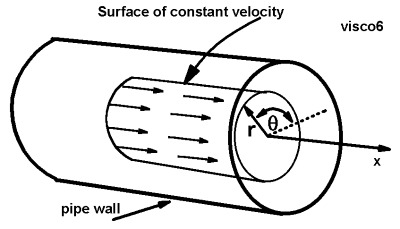
\includegraphics[width=0.5\textwidth]{Figures/pe.jpg}
		\caption{Poiseuille's Flow}
	\end{figure}
\end{english}

\subsection*{معادلة نافير ستوكس المبسطة في الاتجاه \textit{z}}
نبدأ من معادلة نافير ستوكس العامة في الاتجاه $z$ 
\begin{equation}
	\label{eq:generalnavierstokes}
	\rho\left(
	\frac{\partial v_z}{\partial t} + \vec{v} \cdot \nabla v_z 
	\right)
	= - \frac{\partial p}{\partial z} + \mu \nabla^2 v_z
\end{equation}
لكن بالفرضيات التي ذكرناها تصبح المعادلة \eqref{eq:generalnavierstokes}:
\[
\frac{dp }{dz} = \mu \cdot \frac{1}{r} \frac{d}{dr} \left(r \frac{dv_z}{dr}\right)
\]
ولكن $dp/dz$ ثابت لأنه يعتمد فقط على $z$. والسريان غير متغير في $z$. نفرض
\[
\frac{dp}{dz} = \frac{- \Delta p}{L}
\]
حيث 
\begin{itemize}
	\item $\Delta p$ فرق الضغط.
	\item  $L$ طول الانبوب.
\end{itemize}
اذن تصبح المعادلة 
\begin{align}
	\frac{d}{dr} \left(r \frac{dv_z}{dr}\right) = \frac{-\Delta p}{\mu L} r \notag\\
		\label{eq:poiseuillflow}
		r \frac{d^2 v_z}{dr^2} + \frac{dv_z}{dr} =  \frac{-\Delta p}{\mu L} r 
\end{align}
مع الشروط الحدودية
\[
v_z(0) = \text{finite}, \quad v_z(R) = 0
\]
الآن نطبق تحويل لابلاس على \eqref{eq:poiseuillflow} نحصل على
\[
\LL\left\{r \frac{d^2 v_z}{dr^2} + \frac{dv_z}{dr}\right\} = \LL\left\{\frac{-\Delta p}{\mu L} r\right\}
\]
\[
-\frac{d}{ds} \left[s^2 V(s) - s v_z(0) - v_z'(0)\right] + \left[sV(s) - v_z(0)\right] =  \frac{-\Delta p}{\mu L s^2}
\]
\[
-s^2V'(s) -2s V(s) + v_z(0) + sV(s) - v_z(0) = \frac{-\Delta p}{\mu L s^2}
\]
\[
V'(s) + \frac{1}{s} V(s) = \frac{\Delta p}{\mu L s^4}
\]
بإستخدام عامل التكامل 
\[
I(s) = \exp\left(\int \frac{1}{s}\right) = \exp(\ln s) = s
\]
اذن يكون الحل
\[
I(s) V(s) = \int  \frac{\Delta p}{\mu L s^4} I(s)\, ds
\]
\[
s V(s) = \int \frac{\Delta p}{\mu L s^3} \, ds
\]
\[
s V(s) = -\frac{\Delta p}{2\mu L s^2} + C
\]
\[
V(s) = -\frac{\Delta p}{2\mu L s^3} + \frac{C}{s}
\]
بتطبيق لابلاس العكسي
\[
v_z(r) = - \frac{\Delta p}{4\mu L } r^2 + C
\]
بما ان $v_z(R) = 0 $
\[
C = \frac{\Delta p}{4\mu L } R^2
\]
اذن الحل النهائي
\[
v_z(r) = \frac{\Delta p}{4\mu L } (R^2 - r^2)
\]
الآن نستخرج معدل التدفق الحجمي $Q$ بالقانون
\begin{align*}
	Q &= \int_0^R v_z(r) \cdot 2\pi r \, dr\\
	&= \int_{0}^{R} \left(\frac{\Delta p}{4\mu L } (R^2 - r^2)\right)\cdot 2\pi r\, dr
\end{align*}

بالتكامل نحصل على 
\[
Q = \frac{\pi R^4 \Delta p}{8 \mu L}
\]
تسمى هذه المعادلة بقانون بوازوي.\\ \\
\noindent
\textbf{مثال تطبيقي}\\
\noindent
في الاوعية الدموية الصغيرة مثل الشرايين الدقيقة والشعيرات الدموية، يمكن اعتبار الدم كسائل لزج يتدفق تدفق طبقي. هنا نستخدم قانون بوازوي لتقدير معدل تدفق الدم عبر وعاء دموي دائري.\\ \\
\noindent
\textbf{ملاحظات مهمة للتطبيق}
\begin{itemize}
	\item لان $R^4$ موجود في القانون فإن تغيراً بسيطاً في نصف القطر يؤدي الى تغير كبير في معدل التدفق.
	\item مثلاً، اذا تضاعف نصف القطر فإن $Q$ يزيد بمقدار $2^4 = 16$.
	\item  هذا يفسر كيف ان تضيق الشرايين (كما في حالة تصلب الشرايين) يؤدي الى انخفاض حاد في تدفق الدم.
\end{itemize}
\noindent
\textbf{مثال عددي بسيط}\\
نصف القطر $R = 0.001 \text{m}$ ، وفرق الضغط $\Delta p = 100 \text{Pa}$ وطول الانبوب $L = 0.1 \text{m}$ و اللزوجة $\mu = 3 \times 10^{-3} \text{Pa}\cdot \text{s}$ فإن معدل التدفق
\[
Q = \frac{\pi (0.001)^4}{8\times 3\times10^{-3}} \cdot \frac{100}{0.1} \approx 1.31 \, \mu L/s
\]

\section{الحركة التوافقية البسيطة \en{Simple Harmonic Motion}}
الحركة التوافقية البسيطة هي نوع من الحركة التبذبية حيث يتحرك الجسم ذهاباً و اياباً حول موضع اتزان ، وتكون القوة المؤثرة عليه متناسبة طردياً مع الازاحة من موضع الاتزان ، لكنها تعاكسها في الاتجاه ، اي  ان القوة المؤثرة عليه تحقق العلاقة 
\[
F = - k x
\]
حيث $F$ القوة المؤثرة على الجسم و $x$ الازاحة من موضع الاتزان و $k$ ثابت القوة (ثابت النابض في قانون هوك). والاشارة السالبة تعني ان القوة تعاكس اتجاه الزاوية.

\begin{english}
	\begin{figure}[ht]
		\centering
		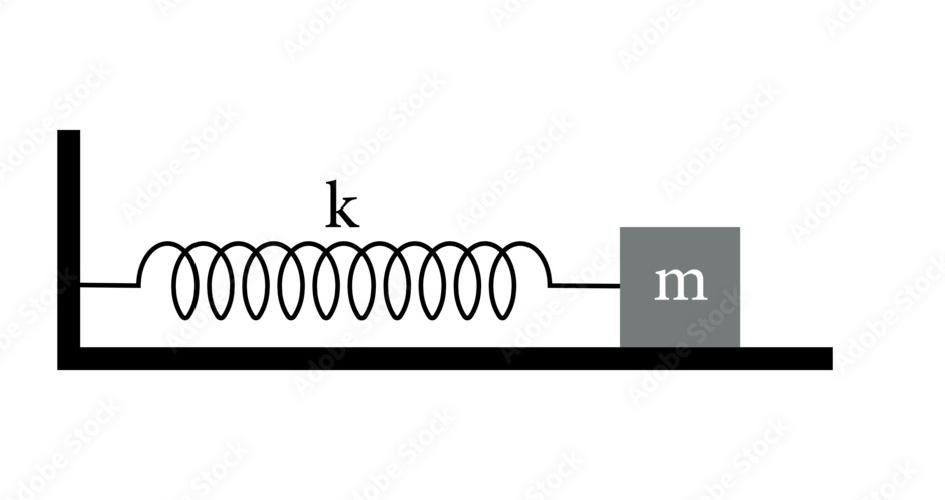
\includegraphics[width=0.5\textwidth]{Figures/shm.jpg}
		\caption{Simple Harmonic Motion}
	\end{figure}
\end{english}

\subsection*{اشتقاق المعادلة التفاضلية}
نبدأ من قانون نيوتن الثاني
\[
F = ma = m \frac{d^2 x}{dt^2}
\]
وبما ان $F = -kx$ ، نكتب
\[
m \frac{d^2 x}{dt^2} = - kx
\]
بالقسمة على $m$
\[
\frac{d^2 x}{dt^2} + \frac{k}{m} x = 0
\]
نسمي $\omega =\sqrt{ k/m}$ ، حيث $\omega$ هو التردد الزاوي. فتصبح المعادلة التفاضلية
\begin{equation}
	\label{eq:shm}
	\frac{d^2 x}{dt^2} + \omega^2 x = 0
\end{equation}
حيث الشروط الابتدائية
\begin{itemize}
	\item $x(0) = x_0$ الازاحة الابتدائية.
	\item $x'(0) = v_0$ السرعة الابتدائية.
\end{itemize}
الآن نطبق تحويل لابلاس على طرفي المعادلة \eqref{eq:shm} نحصل على

\[
\LL\left\{\frac{d^2 x}{dt^2} + \omega^2 x = 0 \right\}
\]
\[
s^2X(s) - sx(0) - x'(0) + \omega^2 X(s)=0
\]
\[
(s^2 + \omega^2 ) X(s) = sx_0 + v_0 
\]
\[
X(s) = x_0\frac{s}{(s^2 + \omega^2 )} + v_0 \frac{1}{s^2 + \omega^2}
\]
بتطبيق لابلاس العكسي نحصل على 
\[
x(t) = x_0\cos(\omega t) + \frac{v_0}{\omega} \sin(\omega t)
\]
يمكن اختزال هذه المعادلة الى 
\[
x(t) = C \cos(\omega t + \phi)
\]
حيث 
\[
C = \sqrt{x_0^2 + \frac{v_0^2}{\omega^2}}, \quad \phi=\tan^{-1} \left(\frac{-v_0}{\omega x_0}\right)
\]
حيث $C$ تسمى السعة للحركة. و $\phi$ زاوية الطور\\ \\
\noindent
\textbf{مثال عددي}\\
جسم كتلته $m = 0.5 \, \text{Kg}$ مربوط بنابض ثابت مرونته $k = 2\, N/m$ عند الزمن $t=0$ كان الجسم على بعد $x_0=0.1\text{m}$ من موضع الاتزان ويتحرك بسرعة ابتدائية $v_0 = 0.2 m/s$ نحو موضع الاتزان. احسب الآتي
\begin{itemize}
	\item التردد الزاوي $\omega$.
	\item موضع الجسم بعد مرور زمن $t = 2\sec$.
	\item السعة $C$ و زاوية الطور  $\phi$.
\end{itemize}
\begin{solution}
	1. التردد الزاوي
	\[
	\omega = \sqrt{\frac{k}{m}} = \sqrt{\frac{2}{0.5}} = 2 \, \text{rad}/\text{s}
	\]
	2. حساب الازاحة. بما ان 
	\[
	x(t) =  x_0\cos(\omega t) + \frac{v_0}{\omega} \sin(\omega t)
	\]
	اذن
	\[
	x(t) =  0.1\cos(2 t) + \frac{0.2}{2} \sin(2 t)
	\]
	نعوض $t=2$
	\[
	x(2) = 0.1 [\cos 4 + \sin 4] \approx  -0.1410 
	\]
	اي ان الجسم عند $t=2 s$ يقع على بعد $0.141$ متر على يسار موضع الاتزان.\\ 
	\noindent
	3. نحسب السعة 
	\[
	C = \sqrt{x_0^2 + \frac{v_0^2}{\omega^2}} = \sqrt{0.01 + \frac{0.04}{4}} \approx 0.1414
	\]
	زاوية الطور
	\[
\phi=\tan^{-1} \left(\frac{-v_0}{\omega x_0}\right) = \tan^{-1} \left(\frac{-0.2}{0.2}\right) = - \frac{\pi}{4}
	\]
\end{solution}